Ocorreu-me que mostrar a sequência de operação do sistema é interessante.

\begin{figure}
    \centering
    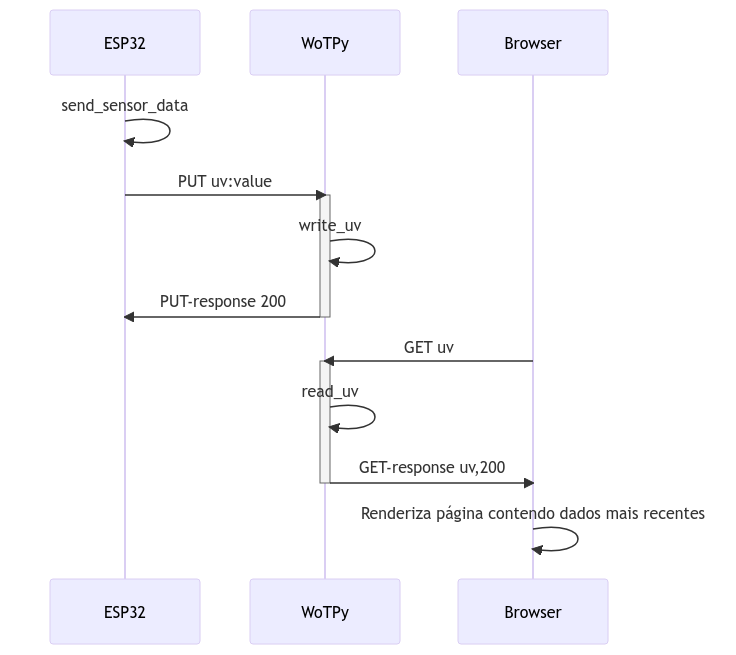
\includegraphics[scale=0.4]{sections/sequencia.png}
    \caption{O dispositivo (ESP32) executa um loop que, a cada 5 segundos executa a função send\_sensor\_data. Esta função envia uma requisição PUT para o servidor (WoTPy). Em resposta a essa requisição o servidor executa o handler (função) write\_uv que contém o envio da resposta. Um usuário pode acessar a informação no servidor através do Browser. Entrar a URL na barra de endereços do Browser o faz enviar ao servidor uma requisição GET. Em resposta à requisição o servidor executa o handler (função) read\_uv, que contém o envio da resposta - no caso, o valor de uv mais recente. O Browser recebe essa informação e renderiza a página contendo a informação.}
    \label{fig:sequencia}
\end{figure}

O servidor é atingido através de seu endereço IP. O dispositivo tem, codificado, o IP do servidor. O Browser também atinge o servidor através do seu IP. 

A especificação do sensor faz parte do código do servidor.

O código do servidor usa WoTPy, que é aderente à recomendação W3C WoT. A recomendação define maneiras de descobrir e configurar \textit{servients}. No caso, o servidor deve ser capaz de configurar-se para receber os dados do dispositivo, desde que o dispositivo envie a informação necessária (no momento a informação está codificada no servidor).

A descoberta do dispositivo pode ser mais complicada porque o dispositivo não usa WoTPy, consequentemente, o programador precisará implementar a funcionalidade sem o auxílio da biblioteca. Uma forma de fazer descoberta automática é através de mDNS (multicast DNS). Esse recurso precisa ser suportado também pelo \textit{Access Point Wi-Fi} e permite que quando um nó da rede envia uma requisição contendo um domínio nomeado, o nome do domínio seja encaminhado para outros nós da rede para resolver o endereço IP que corresponde ao nome. A localização da informação de configuração do \textit{servient} é colocada em uma sub-URL padronizada (por exemplo, wot). Por exemplo, quando um \textit{servient} é iniciado, ele adquire um IP do access point e associa seu nome (internamente codificado) ao IP. Caso uma requisição de solução de nome de domínio lhe chegue, ele responde com seu IP. Caso haja gateways internet no caminho, os gateways que estiverem no caminho da resposta bem sucedida vão manter essa associação, o que acelera o roteamento da informação. Isto só é feito para servidores web, não é feito para clientes. Logo, para o dispositivo poder ser descoberto através desse mecanismo ele precisa ser um servidor web, o que pode não ser possível, dependendo da capacidade computacional e disponibilidade de energia. O ESP32 pode ser configurado como servidor, logo, é compatível com este mecanismo.

Outros mecanismos podem usar diretórios de serviços (servidores possuidores de nome de domínio que mantém tabelas de IPs e características).

O uso (experimentação) dos mecanismos de configuração e descoberta recomendados pela W3C e, em princípio, implementados no WoTPy torna-se possível agora, quando possui-se um \textit{servient} baseado em WoTPy. Esta atividade pode fazer parte das próximas atividades deste TCC. 

% código-fonte para gerar diagrama no editor on-line https://mermaid.live/edit
%sequenceDiagram
%    ESP32->>ESP32: send_sensor_data
%    ESP32->>+WoTPy: PUT uv:value
%    WoTPy->>WoTPy: write_uv
%    WoTPy->>-ESP32: PUT-response 200
%    Browser->>+WoTPy: GET uv
%    WoTPy->>WoTPy: read_uv
%    WoTPy->>-Browser: GET-response uv,200
%    Browser->>Browser: Renderiza página contendo dados mais recentes
